% !TEX encoding = UTF-8
% !TEX TS-program = pdflatex
% !TEX root = ../tesi.tex

%**************************************************************
\chapter{Lo stage}
\label{cap:progettazione}
\label{sec:tecnologie-strumenti}
 \section{La pianificazione}
 \begin{figure}[!h] 
 	\centering 
 	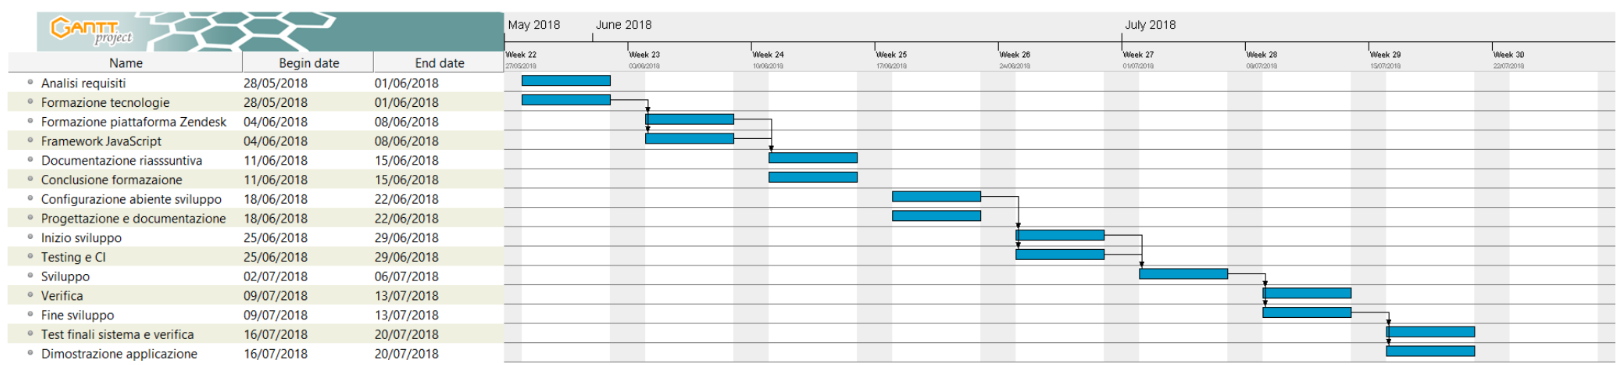
\includegraphics[width=1.2\columnwidth]{piani} 
 	\caption{Diagramma Gantt piano di stage confermato}
 \end{figure}
Per raggiungere gli obiettivi pianificati nel piano di stage e rispettare i
requisiti imposti dall’Università, io e il tutor aziendale abbiamo
previsto 320 ore di lavoro, distribuite in circa 8 settimane da 40 ore ciascuna.
L'inzio è avvenuto il 03 Giugno 2018 e la fine il 03 Agosto 2018, 
terminando cosi con una settimana in ritardo. Le ore fatto comunque rimangono sempre 320(8 settimane), la settimana in più andava a sostituire la settimana libera che mi sono preso dallo stage per le diverse motivazioni personali. 
\\
\\
Le fasi individuate dal piano di studio sono:

\begin{itemize}
	\item \textbf{FASE 1 - Analisi dei requisiti e la formazione tecnica:} durante questa prima fase, dopo diversi incontri con il tutor aziendale verranno definiti tutti i requisiti da soddisfare e le tecnologie da utilizzare al fine di raggiungere l'obiettivo prefissato. Una volta definiti questi concetti, inizierà la formazione e la realizzazione di un semplice \emph{proof of concept}, che andrà a dimostrare quanto imparato e soprattutto la fattibilità dell'applicazione;
	\item \textbf{FASE 2 - La progettazione:} dopo aver individualizzato tutti i requisiti da soddisfare, imparato almeno per una buona parte le tecnologie da utilizzare e realizzato un semplice\emph{ proof of concept}, verrà definita tutta la progettazione architetturale dell'applicazione finale;
		\item \textbf{FASE 3 - Implementazione:} questa fase consiste nella codifica di quanto progettato. E' la fase con la durata più lunga. Tutta l'applicazione deve essere sviluppata in questa fase sia per quanto riguarda il lato frontend che quello backend;
		\item \textbf{FASE 4 - Validazione requisiti e stesura documentazione:} l'ultima fase della pianificazione di durata circa una settimana consiste nel verificare che il \emph{software} realizzato soddisfi tutti i requisiti
			del progetto di stage. Inoltre nello stesso periodo viene redatto la documentazione tecnica, atta a descrivere il progetto realizzato.
\end{itemize}
\section{Analisi dei requisiti e formazione tecnica}
Nei primi giorni ho avuto modo di fare diversi incontri con il tutor aziendale per capire meglio l'applicazione da realizzare e per definire tutti gli obbiettivi da raggiungere. 
Definiti gli obiettivi del progetto, ho iniziato a studiare tutte le tecnologie elencate nel capitolo 3. Ovviamente molte di queste le avevo già studiare nella mia carriera universitaria, ed altre erano molto simili alle tecnologie già viste per conto mio. Quindi non ho avuto tante difficoltà a capire lo \emph{stack} tecnologico da imparare.
 Sono riuscito già alla terza settimana a realizzare il \emph{proof of concept} senza troppe difficoltà.
 \newpage  
\section{La Progettazione}

Di seguito vengono illustrate le strategie di progettazione adottate per la realizzazione del prodotto in questione. La progettazione viene descritta ad alto livello senza descrivere in dettaglio tutti i diagrammi delle classi.
\subsection{Progettazione Frontend}
\label{sec:progettazione}
Come prima cosa sono stati realizzati utilizzando \emph{Figma} i prototipi delle pagine da creare. In questo modo è stato possibile capire sin da subito la struttura delle pagine, rendendo cosi molto semplice la progettazione architetturale di tale pagine.
\subsubsection{Pagina contenente l'editor}
Questa pagina contiene l'editor \emph{drag and drop}. Per creare la struttura di questa pagina sono stati studiati diversi editor online che forniscono le stesse funzionalità(in diversi contesti). Dopo una attenta analisi delle strutture dei diversi editor online è stato concepita la seguente struttura:
\begin{figure}[!h] 
	\centering 
	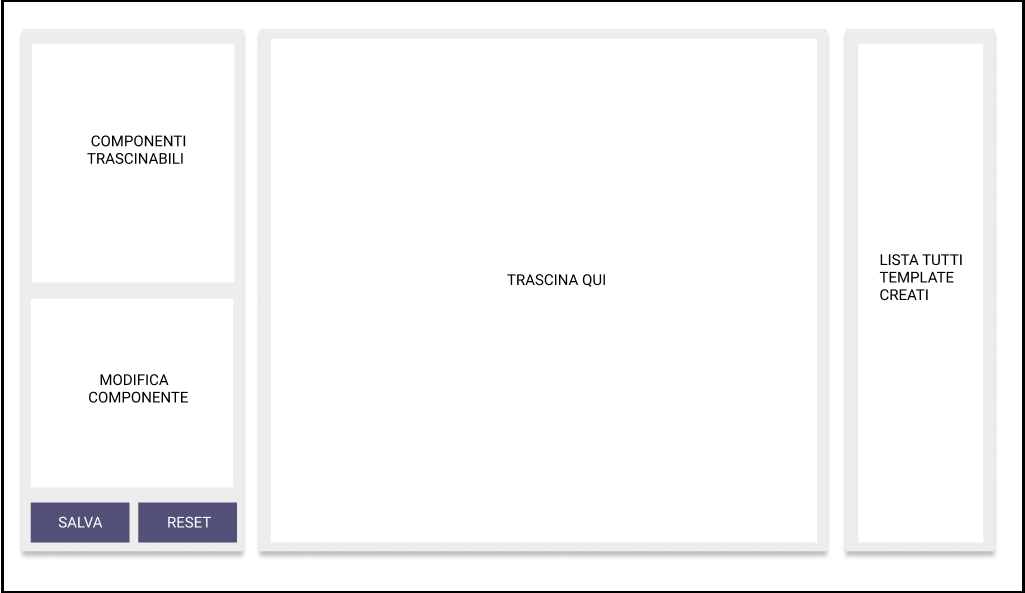
\includegraphics[width=0.9\columnwidth]{mock/mockeditor} 
	\caption{Mock pagina contenente l'editor}
\end{figure}  
\\
\begin{itemize}
	\item Il primo contenitore in alto a sinistra dovrà contenere tutti i componenti trascinabili. Ogni elemento rappresenta uno specifico tipo di oggetto HTML e CSS, come ad esempio il testo, banner, titolo, immagine ecc;
	\item Il secondo contenitore a sinistra contiene tutte le proprietà modificabili per ogni elemento;
	\item Il contenitore in centro(container) rappresenta la zona dove tutti gli elementi vengono trascinati. In questo contenitore viene visualizzato a schermo il contenuto HTML e CSS di ogni elemento trascinato. Inoltre dovrà essere possibile modificare tale contenuto ed eliminare un elemento se necessario;
	\item Il contenitore a destra dovrà contenere tutti i template realizzati dagli utenti. Quindi esso contiene semplicemente una lista di tutti i template.  
\end{itemize}

\subsubsection{Pagina contenente il widget} Questa pagina contiene una semplice lista che dovrà contenere tutti i template da visualizzare nella pagina dei \emph{tickets}, in modo che essi possono essere scelti dagli agenti di Zendesk.
\\ 
\subsubsection{Pagina login}
Semplice pagina contenete il \emph{form} per il login. Una volta inseriti i valori validi l'utente sarà utenticato come amministratore, caricandoli cosi la pagina degli amministratori. 
\begin{figure}[!h] 
	\centering 
	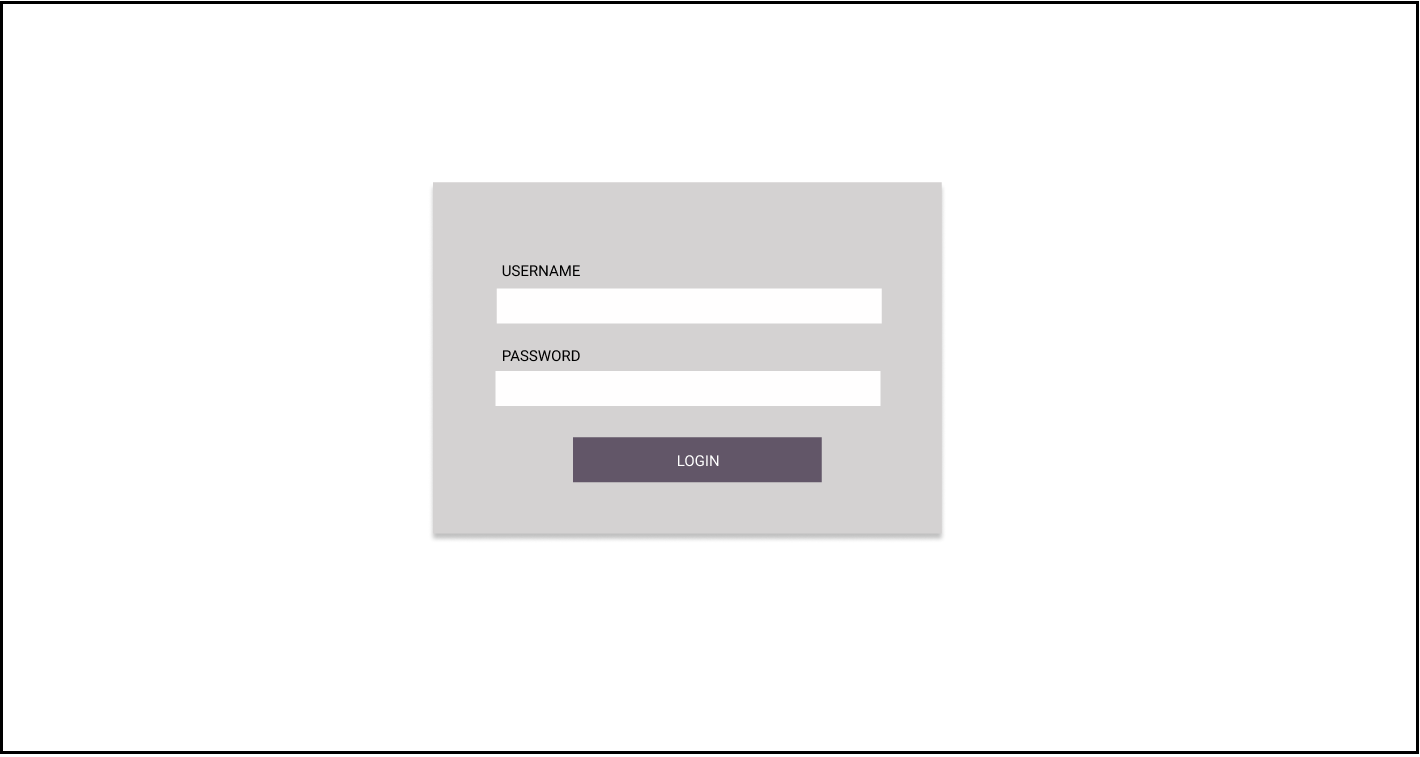
\includegraphics[width=1\columnwidth]{mock/mocklogin} 
	\caption{Mock pagina di login}
\end{figure}  \newpage
\subsubsection{Pagina degli amministratori}
Questa pagina dovrà essere realizzata per gli amministratori di Nextep, per permettere a loro di gestire tutti i clienti utilizzatori dell'applicazione. 
\begin{figure}[!h] 
	\centering 
	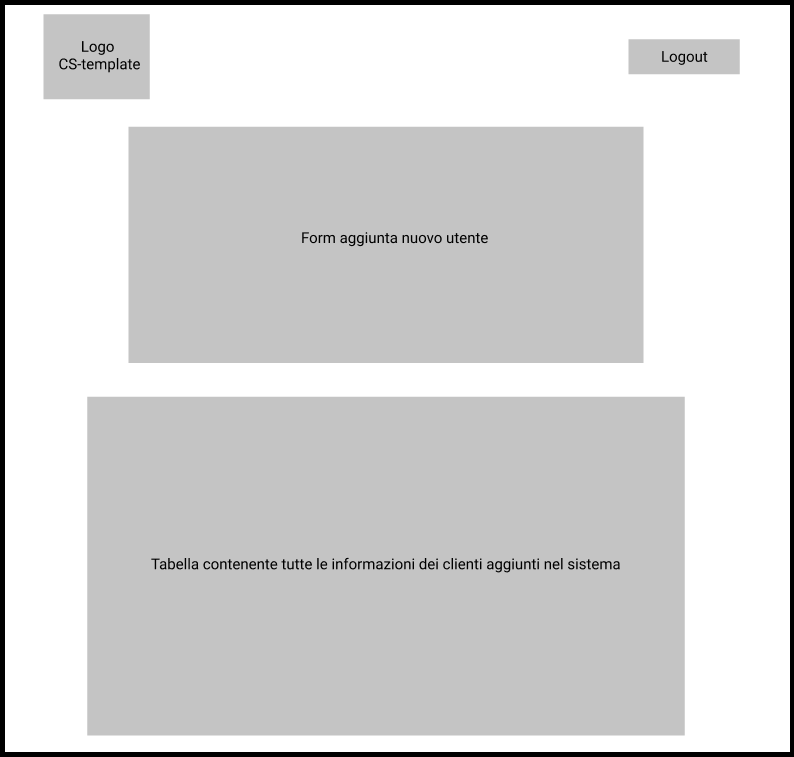
\includegraphics[width=0.8\columnwidth]{mock/mockadmin} 
	\caption{Mock pagina degli amministratori}
\end{figure}  
\begin{itemize}
	\item Contiene un semplice form per aggiungere un nuovo cliente;
	\item Contiene una semplice tabella, dove ogni elemento della tabella contiene le informazioni di un singolo cliente.
\end{itemize}\newpage
\subsubsection{Struttura applicazione}
Essendo un'unica applicazione che contiene sia le pagine degli amministratori di Nextep che le pagine dell'applicazione Zendesk, si è pensato quindi una struttura illustrata nel seguente diagramma.
\begin{figure}[!h] 
	\centering 
	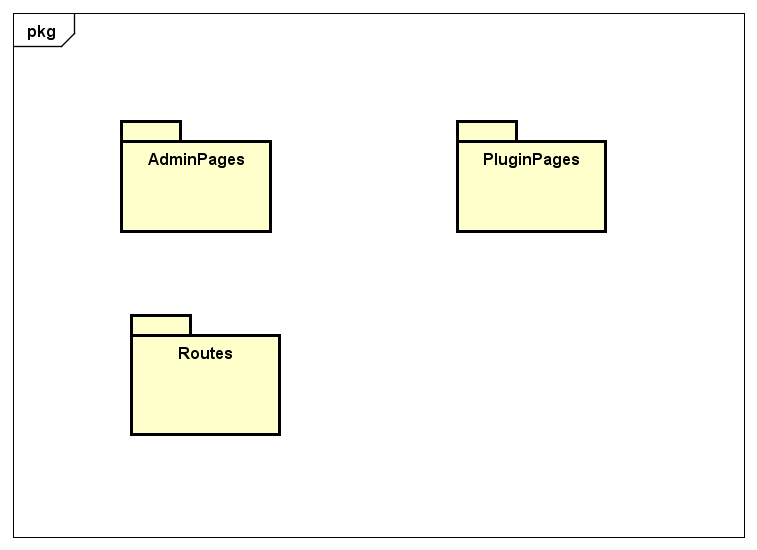
\includegraphics[width=0.8\columnwidth]{prog/pack} 
	\caption{Struttura applicazione}
\end{figure}
\begin{itemize}
	\item \textbf{AdminPages:} contiente tutti i componenti e i servizi\footcite{Nel Appendice si trova una descrizione completa di un servizio Angular} che vanno a formare le pagine(login e di amministratori) per gli utenti di Nextep;
	\item \textbf{PluginPages:} contiene tutti i componenti e i servizi per la pagine contenente l'editor e la pagina contenenti il widget;
	\item \textbf{Routes:} contiene tutto il codice per la gestione della navigazione dell'applicazione.
\end{itemize}
\begin{figure}[!h] 
	\centering 
	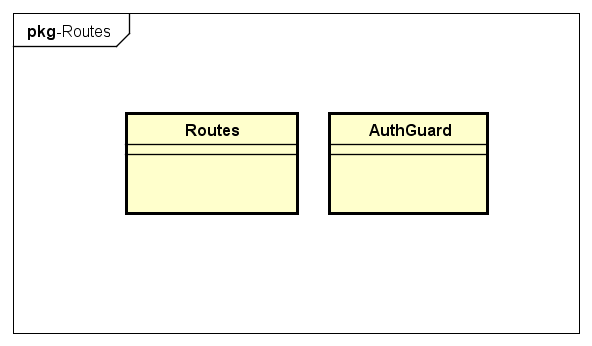
\includegraphics[width=0.6\columnwidth]{prog/routes} 
	\caption{Struttura Routes}
\end{figure}
\begin{itemize}
	\item L'oggetto \textbf{Routes} contiene un array di tutte le navigazioni dell'applicazione,
	\item L'oggetto \textbf{AuthGuard} serve per bloccare la navigazione alla pagina degli amministratori finchè l'utente non effettua il login. 
	\\
\end{itemize}
\subsubsection{PluginPages}
Contiene tutti i componenti e servizi per realizzare le pagine contenenti l'editor e il widget.
\begin{figure}[!h] 
	\centering 
	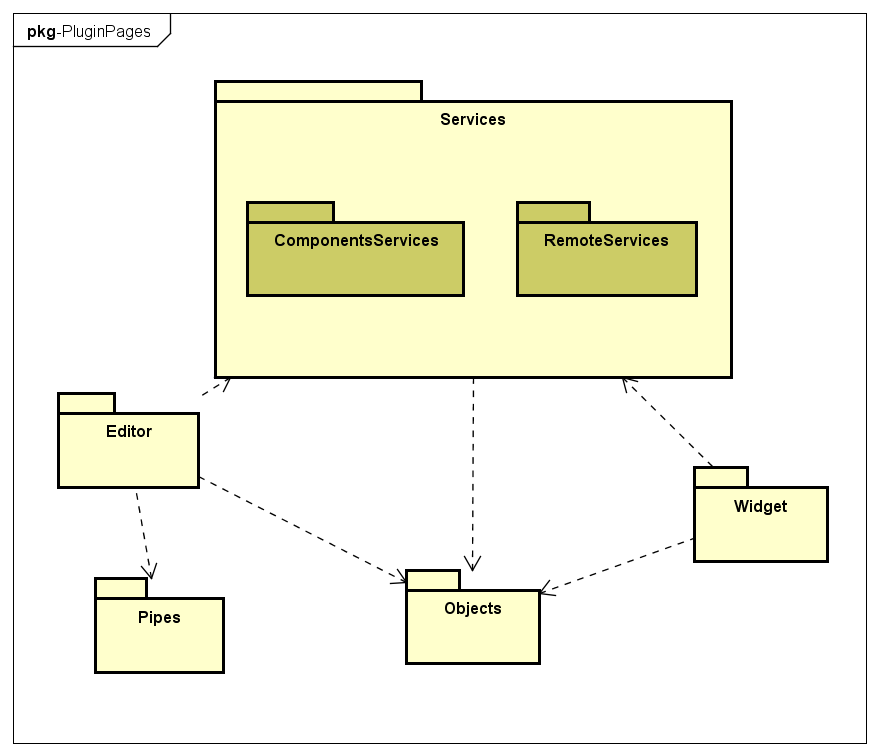
\includegraphics[width=0.8\columnwidth]{prog/pluginpages} 
	\caption{Struttura PluginPages}
\end{figure}
\begin{itemize}
	\item \textbf{ComponentsServices:} contiente tutti i servizi che permettono di scambiare i dati tra i componenti locali;
	\item \textbf{RemoteServices:} contiene tutti i servizi utilizzati per comunicare con il lato backend dell'applicazione. Quindi principalmente per leggere, aggiungere o rimuovere i template dal database su AWS;
	\item \textbf{Objects:} contiene tutti i tipi creati per rappresentare diversi tipi di dati;
	\item \textbf{Editor:} contiene tutti i componenti Angular che formano le pagine contenenti l'editor;
	\item \textbf{Widget:} contiene tutti i componenti Angular che formano le pagina contenenti il widget;
	\item \textbf{Pipes:} contiene le pipes di  Angular.
\end{itemize}
\newpage
\subsubsection{AdminPages}
Contiene tutti i componenti e servizi per realizzare la pagina di login e la pagina degli amministratori.
\begin{figure}[!h] 
	\centering 
	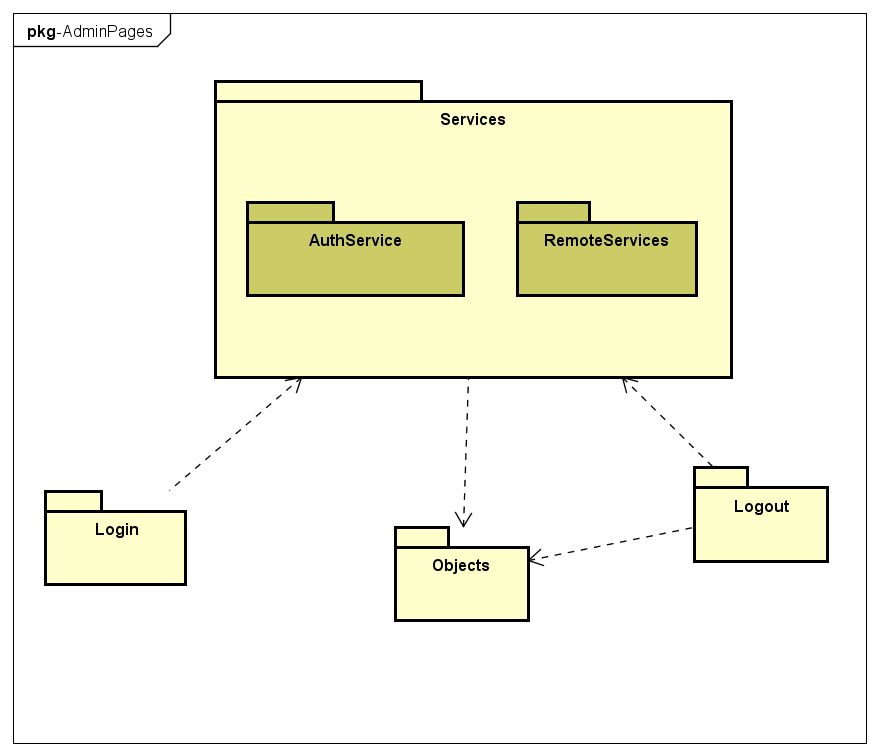
\includegraphics[width=0.8\columnwidth]{prog/adminpages} 
	\caption{Struttura AdminPages}
\end{figure}
\begin{itemize}
	\item \textbf{AuthService:} contiene il servizio che permette di effetuare il login;
	\item \textbf{RemoteServices:} contiene i servizi per aggiungere, leggere o rimuovere i clienti dal database presente su AWS;
	\item \textbf{Objects:} contiene tutti i tipi creati per rappresentare diverse tipologie di dati;
	\item \textbf{Admin:} contiene tutti i componenti Angular che formano la pagina degli amministratori;
	\item \textbf{Login:} contiene tutti i componenti Angular che formano la pagina di login;
\end{itemize}
\newpage
\subsubsection{Atomic design}
Per realizzare le diverse pagine dell'applicazione è stato utilizzato il concetto di Atomic Design.
Creata da Brad Frost nel 2013, l'Atomic design è una metodologia composta da 5 differenti fasi, utile per creare un sistema di interfacce in maniera gerarchica. In questa metologia si parte dai componenti piu basilari possibili, fino ad arrivare alle pagine finali. E' quindi un approccio bottom-up.
\begin{figure}[!h] 
	\centering 
	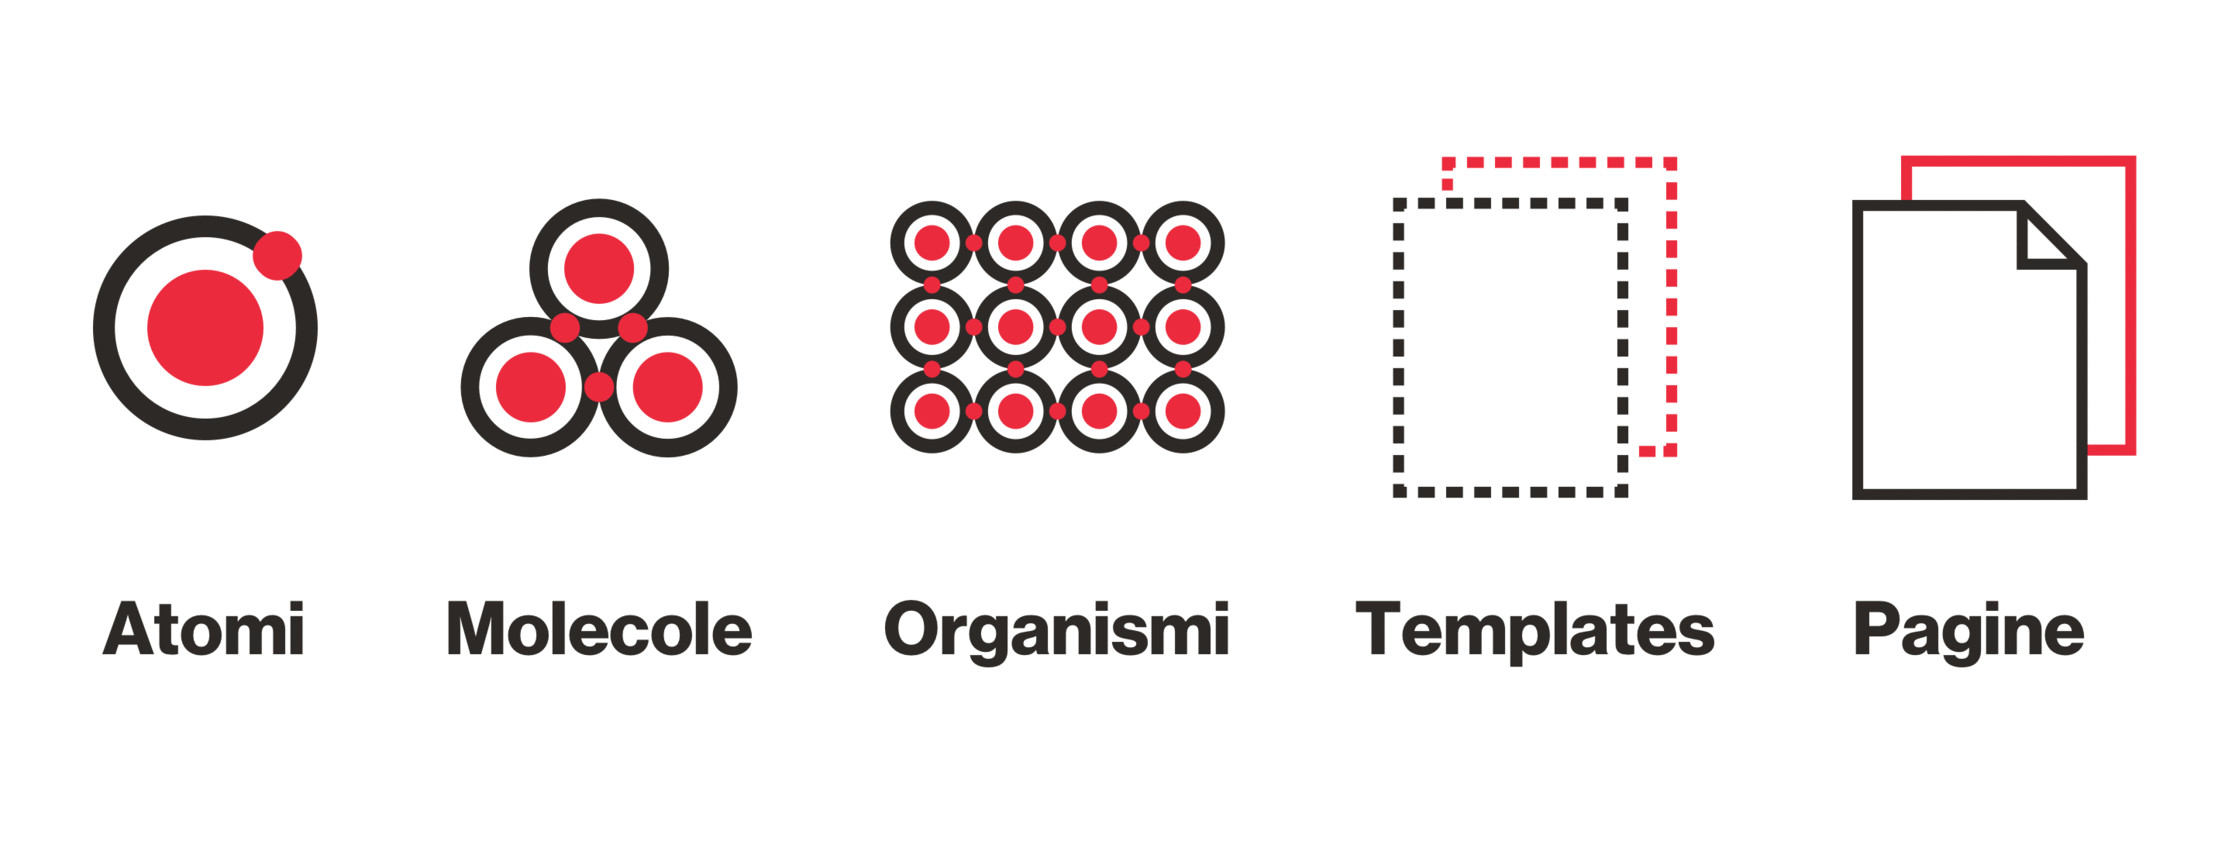
\includegraphics[width=0.8\columnwidth]{atomic} 
	\caption{Elementi atomic design}
\end{figure}
\\

\textbf{Atomi:} in fisica un atomo è la più piccola particella di un elemento che non subisce alterazioni nelle trasformazioni chimiche; nell’Atomic Design gli atomi sono i blocchi fondamentali che comprendono tutta l’interfaccia.
Questi atomi comprendono elementi HTML come tipografia, palette colori, input, bottoni e altri elementi che non possono essere suddivisi ulteriormente senza cessare di essere funzionali.
\\

\textbf{Molecole:} sono semplici gruppi di elementi d'interfaccia che funzionano uniti. Quando combiniamo due oppure più atomi, creiamo quindi una molecola.
\\

Nel contesto dell'applicazione gli atomi e le molecole sono rappresentate dagli elementi della libreria Angular Material, che successivamente sono utilizzati per realizzare l'intera interfaccia dell'applicazione.

\begin{figure}[!h] 
	\centering 
	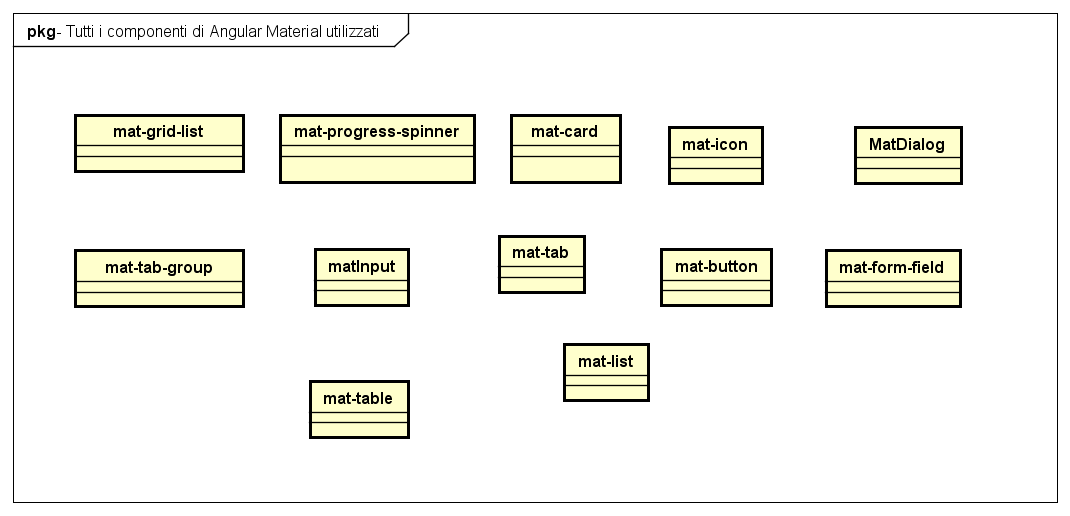
\includegraphics[width=0.8\columnwidth]{prog/angular} 
	\caption{Componenti Angular Material che formano gli atomi e le molecole dell'applicazione}
\end{figure} 
\newpage
\textbf{Gli organismi:} sono dei componenti più o meno complessi, composti da gruppi di molecole e/o atomi e/o altri organismi. Questi organismi creano diverse sezioni all'interno della nostra interfaccia. Un esempio può essere un menu di navigazione, che è formato in media da diversi pulsanti/link. 
\\

\textbf{I templates:} sono creati dall'insieme dei nostri atomi, molecole ed organismi creando così la prima idea dello scheletro della pagina.
\\

\textbf{Le pagine:} sono dei templates riempiti di contenuto reale, come immagini, testi, elementi grafici, advertising, ecc. Una pagina quindi è formata da molti template. 
\newpage
\subsection{Progettazione Backend}
\subsubsection{Archittetura serverless}
Il backend dell'applicazione è realizzato utilizzando i servizi web di Amazon, i servizi scelti sono stati descritti nel capitolo 2. In questa sezione viene descritto come questi servizi comunicano tra di loro. La seguente immagine mostra la panoramica dell'archittettura della applicazione Zendesk realizzata(per la pagina degli amministratori la situazione è leggermente diversa). L'immagine descrive come un template viene caricato nel database NoSQL(database non relazionale) presente su Amazon. 
\begin{figure}[!h] 
	\centering 
	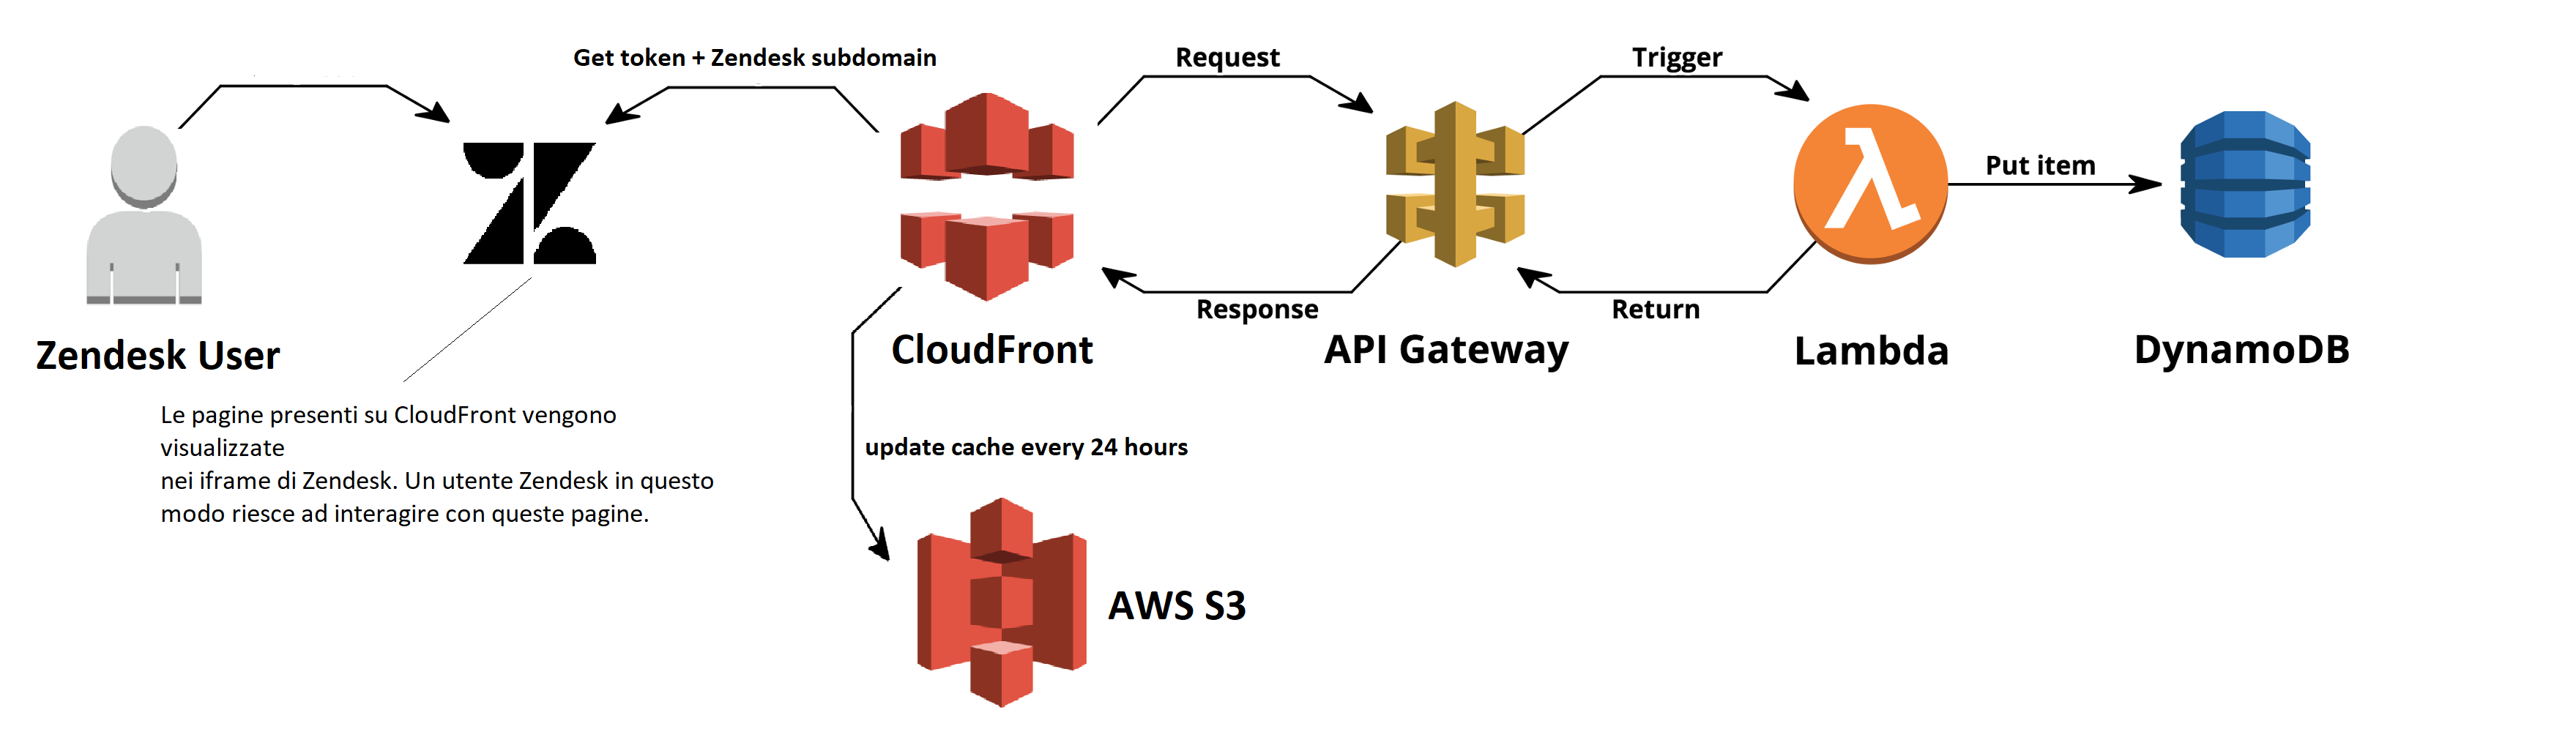
\includegraphics[width=1.2\columnwidth]{prog/zen-architecture} 
	\caption{Flusso completo dell'architettura}
\end{figure} 
\\
\begin{itemize}
	\item Zendesk User interagisce con l'applicazione tramite l'interfaccia di Zendesk;
	\item Le pagine dell'applicazione Angular sono caricate da CloudFront sugli iframe presenti su Zendesk;
	\item Le pagine appena caricate negli iframe leggono il token e il nome del sotto dominio della piattaforma in cui si trovano utilizzando l'oggetto ZAFClient(descritto nel capitolo 2);
	\item Utente crea un nuovo template e lo salva;
	\item L'editor manda la richiesta all'API Gateway, inviando nel header della richiesta il token e il nome del dominio in cui si trova;
	\item API Gateway come prima cosa verifica il token e il nome del sotto dominio se sono validi. Se sono validi genera un evento che innesca una funzione lambda, altrimenti(token e nome dominio non validi) ritorna un messaggio d'errore;
	\item La funzione lambda riceve dati dall'evento generato dall'API Gateway. Utilizzando AWS-SDK interagisce con il database NoSQL e salva il nuovo item(template).
	\item Funzione lambda ritorna un messaggio di successo;
\end{itemize}\newpage
\subsubsection{Architettura pagina degli amministratori}
Il backend cambia leggermente per quanto riguarda la pagina degli amministratori di Nextep. Per accedere a questa pagina bisogna effettuare il login, il quale è stato implementato utilizzano il servizio Cognito che permette di gestire un pool di utenti in maniera molto semplice. La seguente immagine descrive il funzionamento di questa pagina. 
\begin{figure}[!h] 
	\centering 
	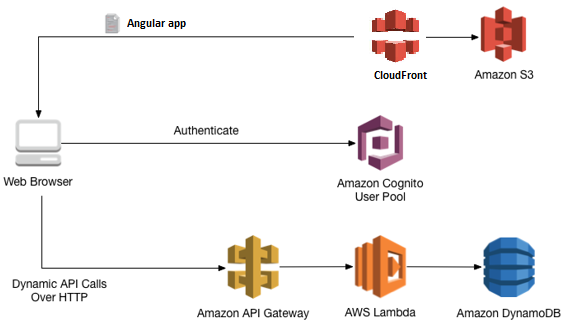
\includegraphics[width=1\columnwidth]{prog/admin-arch} 
	\caption{Flusso completo dell'architettura pagina admin}
\end{figure} 
\begin{itemize}
	\item La pagina di login viene caricata nel browser;
	\item L'utente inserisce le sue credenziali corrette per effettuare il login;
	\item AWS Cognito verifica le credenziali, se sono valide ritorna il token di accesso altrimenti un errore;
	\item Le credenziali sono valide, l'utente accede alla pagina degli amministratori;
	\item L'utente ora può comunicare con l'API Gateway inviando il token ritornato da AWS Cognito. Questo token permette all'utente di inserire oppure eliminare utenti dal database NoSQL presente su AWS;
	\item L'inserimento oppure l'eliminazione di un cliente esegue lo stesso flusso visto sopra per i template. Eccezione fatta per l'AWS Cognito, la pagina degli amministratori ha la stessa architettura.
\end{itemize}
\newpage
\section{Codifica}

Una volta progettata l’architettura 
si passa all’effettiva implementazione dell'applicazione.
 Questa fase è stata quella con la durata più lunga, c'erano tante tecnologie da utilizzare e tanti componenti da realizzare. Inoltre anche tutta la parte backend e soprattutto la questione legata alla sicurezza ha richiesto molto più tempo di quanto previsto. Nel paragrafo qui sotto viene mostrato l'applicazione una volta termina la codifica, spiegando come l'utente interagisce con l'applicazione. 

\subsection{Prodotto realizzato}
\label{cap:progetto-terminato}
Di seguito verrà spiegato in dettaglio come avviene l’interazione dell'utente Zendesk con l'applicazione
Zendesk e dell'utente Nextep con la pagina degli amministratori.

\subsubsection{Editor}
Una volta installata l'applicazione sulla piattaforma Zendesk viene visualizzata automaticamente l'icona dell'applicazione nella \emph{sidebar} della piattaforma. 
\begin{figure}[!h] 
	\centering 
	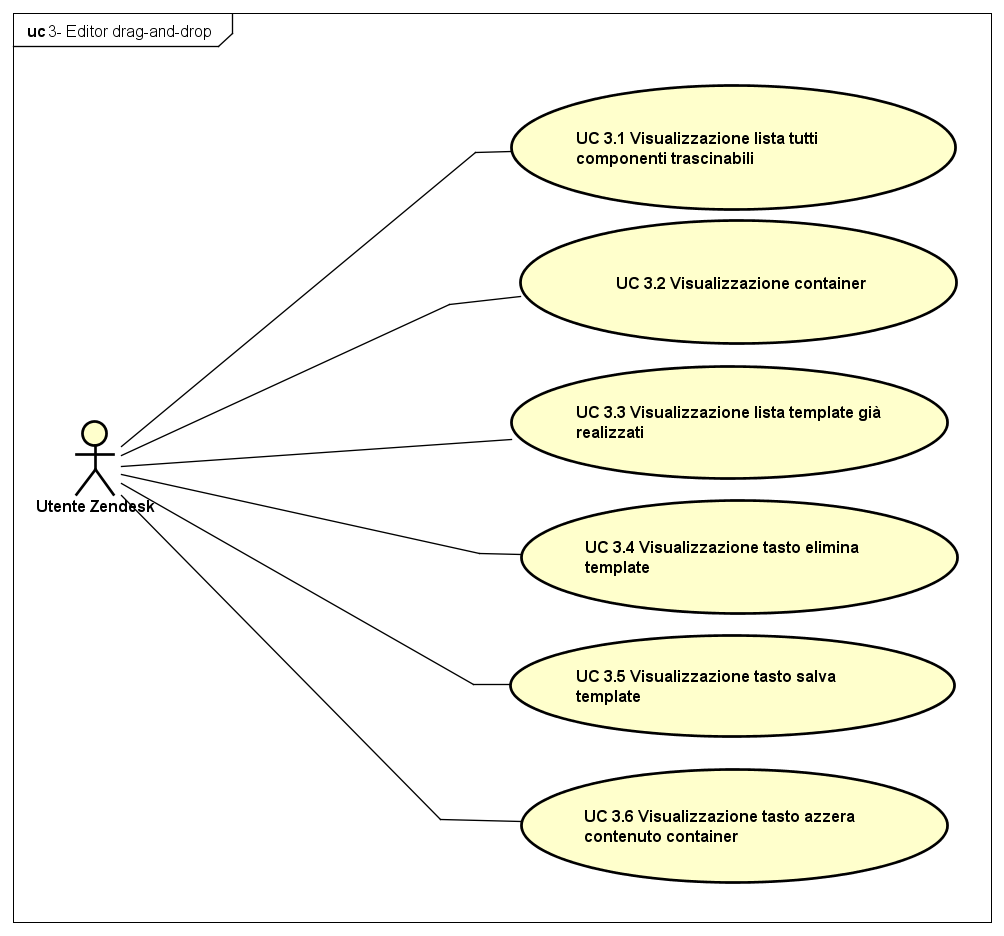
\includegraphics[width=1.2\columnwidth]{editor} 
	\caption{Editor realizzato }
\end{figure}
\begin{itemize}
	\item L'utente può trascinare qualsiasi elemento presente nei "componenti" nel \emph{container} centrale;
	\item Il \emph{container} visualizza a schermo il contenuto  HTML e CSS di ogni elemento trascinato in esso;
	\item Facendo doppio click su qualsiasi elemento presente nel \emph{container} centrale è possibile modificare il suo contenuto oppure eliminarlo dal \emph{container};
	\item Gli elementi nel \emph{container} possono essere ordinati in qualsiasi modo semplicemente facendo \emph{drag-and-drop};
	\item E' possibile azzerare il contenuto del \emph{container} semplicemente cliccando il pulsante "Azzera";
	\item Una volta realizzato il template desiderato l'utente può salvarlo cliccando il pulsante "Aggiungi". Verrà chiesto all'utente di inserire il nome del template, inserendo il nome valido il template verrà automaticamente salvato sul database NoSQL di Amazon;
	\item A destra nell' "Elimina template" è possibile visualizzare tutti i template realizzati e se necessario eliminarli semplicemente cliccano sull'icona "X".  
\end{itemize}
\subsubsection{Widget} 
Il widget permette all'agente di Zendesk di utilizzare i template realizzati nelle risposte verso clienti. 
\begin{figure}[!h] 
	\centering 
	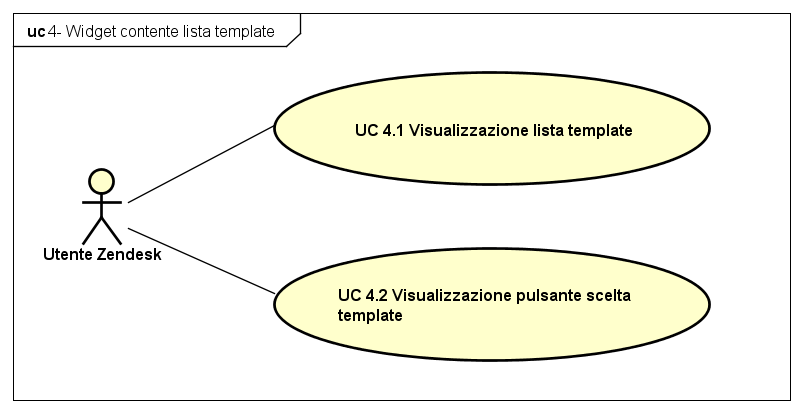
\includegraphics[width=1.2\columnwidth]{widget} 
	\caption{Widget realizzato }
\end{figure}
\begin{itemize}
	\item L'utente visualizza nel widget tutti i template realizzati;
	\item L'utente può selezionare il template da utilizzare nella risposta;
	\item Il template viene automaticamente aggiunto alla risposta. 
\end{itemize}
\newpage
\subsubsection{Pagina di login}
Nell'immagine di seguito viene visualizzato il \emph{form} di login contenuto nella pagina di login. Una volta inseriti i dati corretti, viene automaticamente caricata la pagina degli amministratori. Se i dati inseriti non sono corretti, viene mostrato a schermo un messaggio di errore.
\begin{figure}[!h] 
	\centering 
	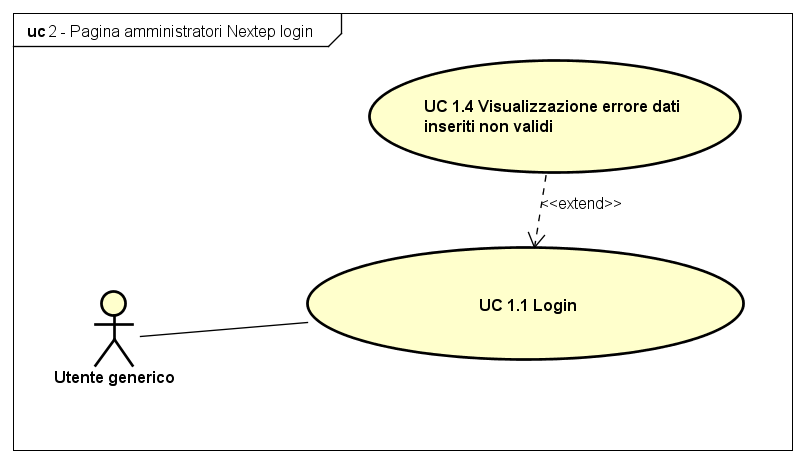
\includegraphics[width=0.8\columnwidth]{login} 
	\caption{Form login }
\end{figure}
\subsubsection{Pagina degli amministratori}
Nell'immagine di seguito viene visualizzata la pagina degli amministratori. In questa pagina è possibile aggiungere e rimuovere un cliente di Nextep che utilizza oppure andrà ad utilizzare l'applicazione CS-Template.
\begin{figure}[!h] 
	\centering 
	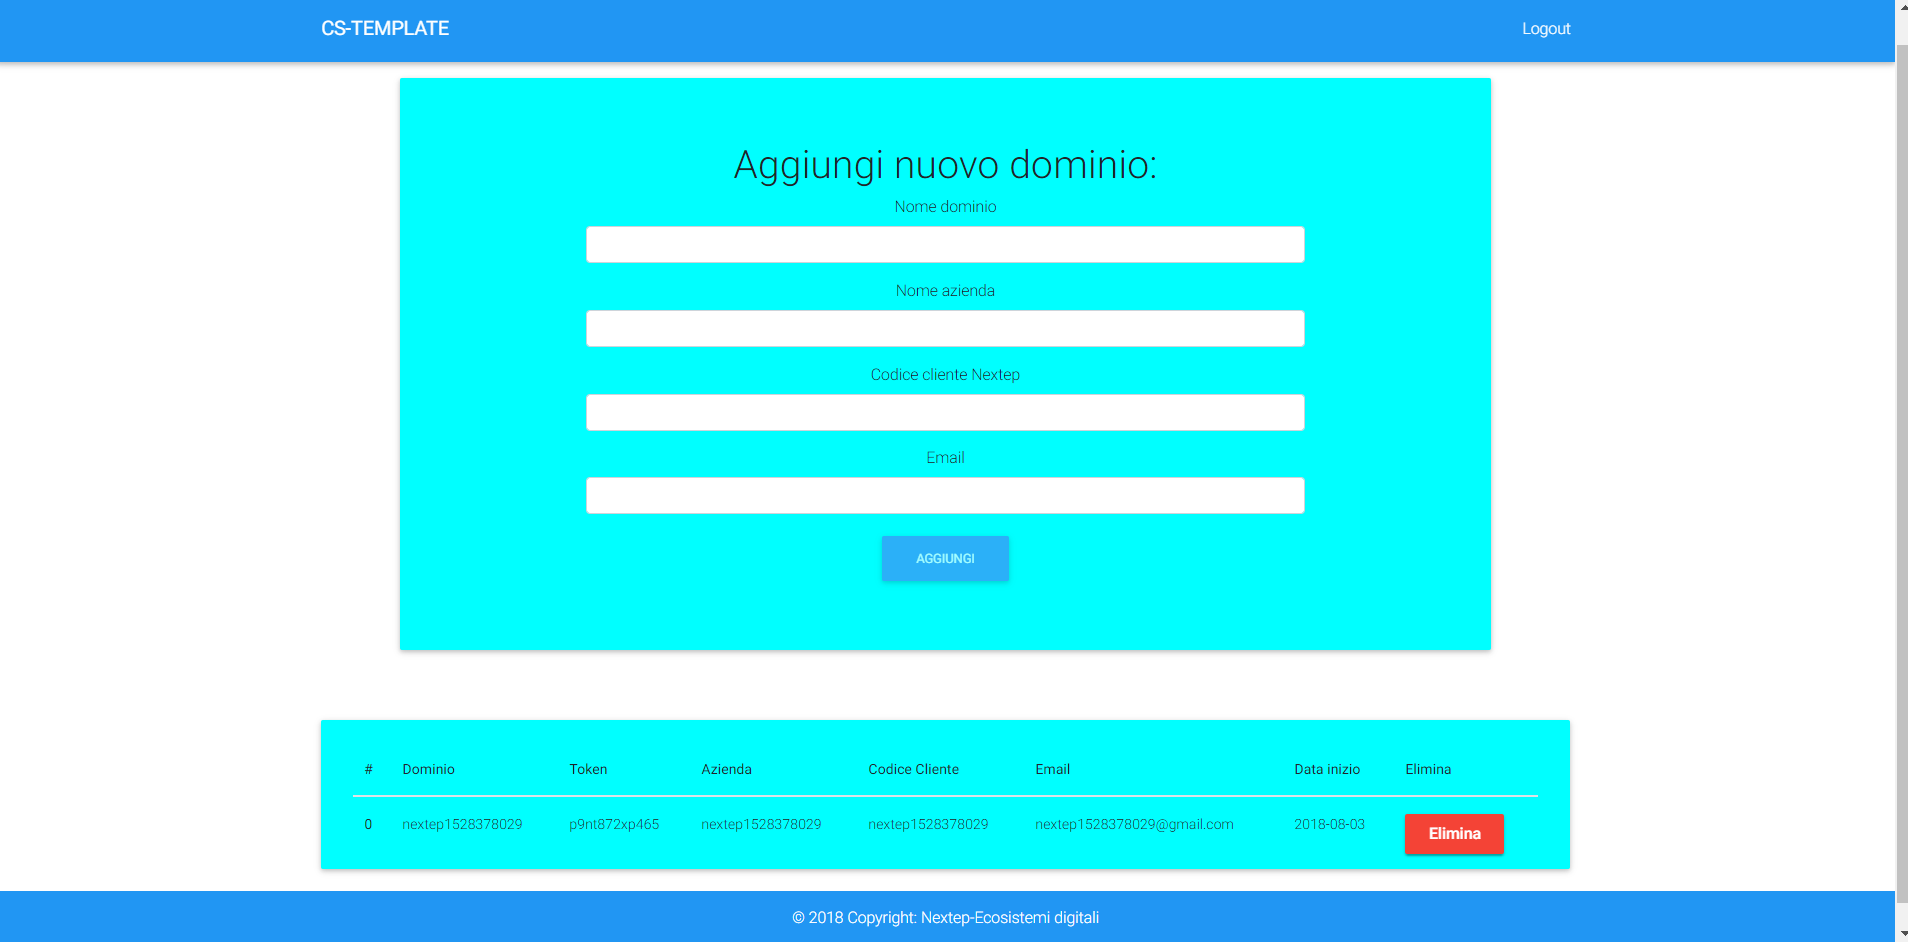
\includegraphics[width=1.2\columnwidth]{admin} 
	\caption{Pagina degli amministratori }
\end{figure}

\section{Validazione} 
Terminata la codifica sono stati eseguiti molti test per verificare che il prodotto realizzato soddisfi tutti i requisiti definiti. Nelle ultime settimane sono stati fatti molti test, provando l'applicazione su quasi tutti i browser più famose, in modo da verificare il corretto funzionamento in tutte le circostanze. Una volta finita la validazione negli ultimi giorni è stata realizzata tutta la documentazione che permettesse agli sviluppatori di Nextep di capire in dettaglio come l'applicazione è stata realizzata. Alla fine tutto il realizzato è stato caricato in modo più ordinato possibile nella repository Gitlab dell'azienda Nextep.

\begin{figure}[!h] 
	\centering 
	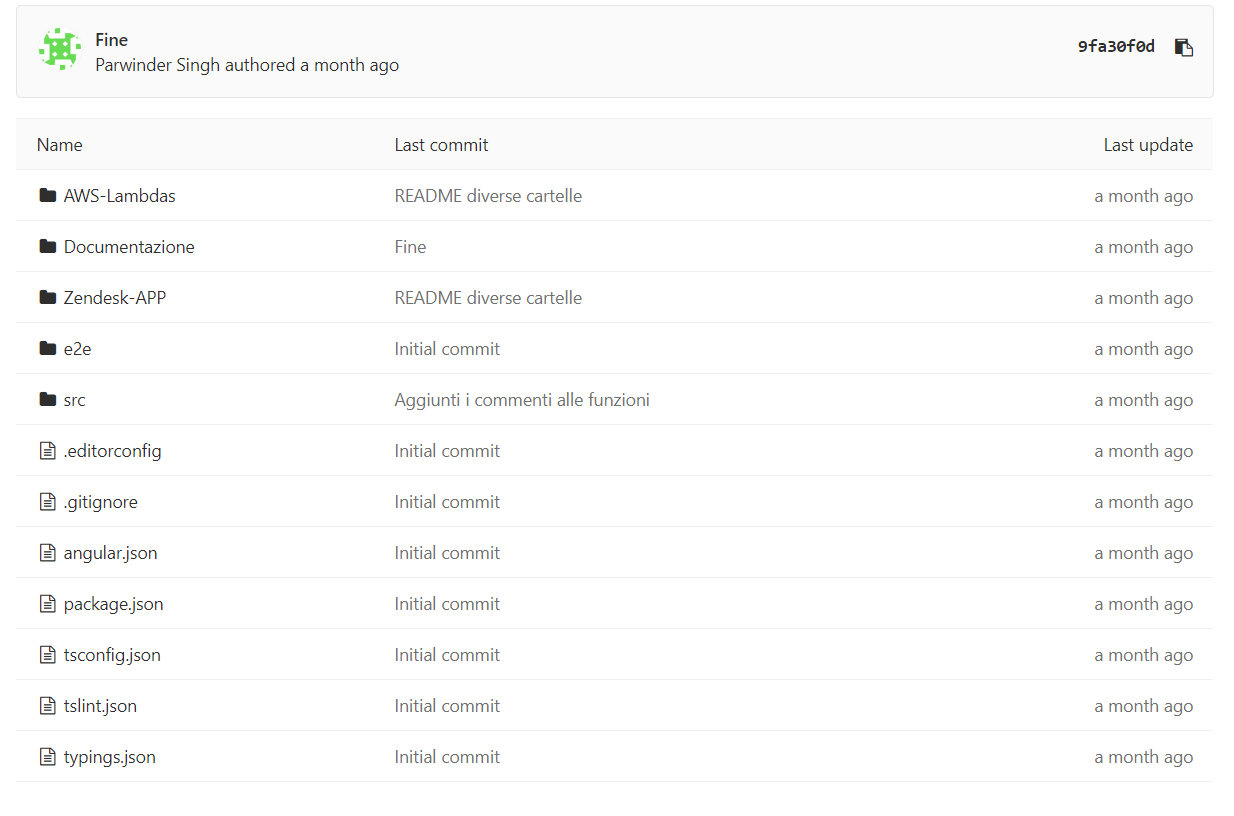
\includegraphics[width=1\columnwidth]{gitlab2} 
	\caption{Repository Gitlab fine progetto }
\end{figure} 